\documentclass{elegantbook}
\usepackage[square,numbers,sort&compress]{natbib}
\newcommand{\upcite}[1]{\textsuperscript{\textsuperscript{\cite{#1}}}}
\usepackage{multirow}
\usepackage{color}
\usepackage{tikz}
\usetikzlibrary{shapes.geometric, arrows}
\tikzstyle{startstop} = [rectangle, rounded corners, minimum width = 2cm, minimum height=1cm,text centered, draw = black, fill = red!40]
\tikzstyle{acti} = [rectangle, trapezium left angle=70, trapezium right angle=110, minimum width=5cm, minimum height=0.5cm, text centered, draw=black, fill = blue!40]
\tikzstyle{pool} = [rectangle, trapezium left angle=70, trapezium right angle=110, minimum width=2cm, minimum height=0.5cm, text centered, draw=black, fill = purple!40]
\tikzstyle{process} = [rectangle, minimum width=3cm, minimum height=1cm, text centered, draw=black, fill = green!50]
\tikzstyle{conv} = [rectangle, minimum width=3cm, minimum height=1cm, text centered, draw=black, fill = magenta!50]
\tikzstyle{loss} = [rectangle, rounded corners, minimum width = 2cm, minimum height=1cm,text centered, draw = black, fill = yellow!40]
\tikzstyle{arrow} = [->,>=stealth]

% title info
\title{Deep Learning}
\subtitle{MNIST Digits Classification with CNN}
% bio info
\author{Yantian Luo}
\institute{Electronic Engineering}
\version{2018310742}
\date{\today}
\logo{logo.png}
\cover{cover.jpg}

\begin{document}

\maketitle
\tableofcontents
\mainmatter
\hypersetup{pageanchor=true}
% add preface chapter here if needed
\chapter{Introduction}
MNIST digits dataset is a widely used database for image classification in machine learning field. It contains 60,000 training samples and 10,000 testing samples. Each sample is a $784\times1$ column vector, which is transformed from an original $28\times28$ pixels grayscale image.

In this homework, we will continue working on MNIST digits classification problem by utilizing convolutional neural network (CNN). The main challenge is to implement the forward and backpropagation functions of convolutional layer and pooling layer from scratch! And at last, we compare the the difference of results you obtained when working with MLP.

\chapter{Algorithm Design}
In this homework, we have basis about the Linear layer, Relu layer, Sigmoid layer, EuclideanLoss and SoftmaxCrossEntropyLoss from homework1, thus we don't need to complete their forward and backward functions another time. Therefore, the most important challenge for us is to implement the forward and backpropagation functions of convolutional layer and
pooling layer.



\chapter{Experients and Results}

In this chapter, we use CNN to work on MNIST digits classification problem and get the accuracy and loss, and we compare the difference of results obtained when working
with MLP in homework1. And at last, we visualize the first convolution layer's output after ReLU for 0-9 digit images.

\section{Experiments1 (two conv layers + one linear layer)}
The network structure in this section is designed as Figure \ref{fig1} and training arguments is as follow:

\begin{lstlisting}[frame=single,language=python]  
config = {
	'learning_rate': 0.01,
	'weight_decay': 0.0001,
	'momentum': 0.9,
	'batch_size': 100,
	'max_epoch': 100,
	'disp_freq': 50,
}
\end{lstlisting}

\begin{figure}[htbp]
	\centering
	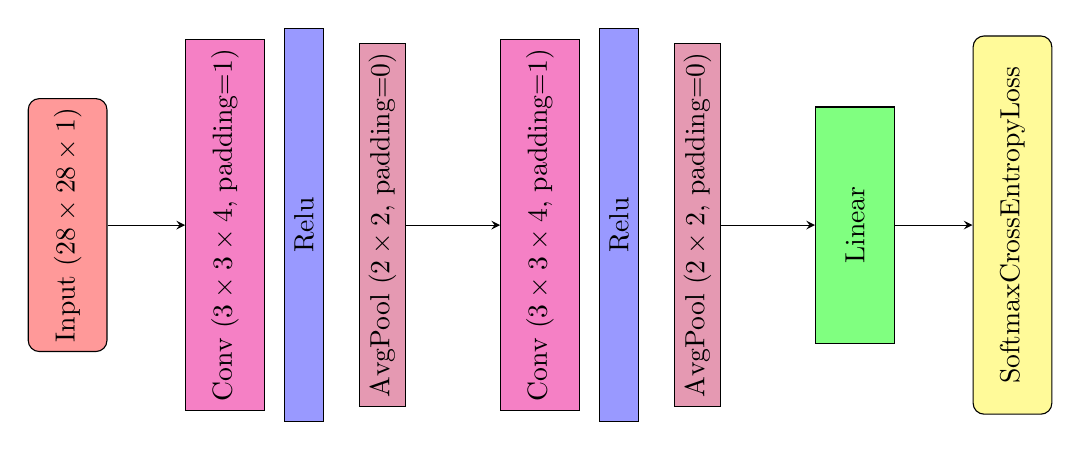
\begin{tikzpicture}
		\node (start) [startstop, rotate=90] {Input ($28\times28\times 1$)};
		\node (conv1) [conv, rotate=90, below of=start, yshift=-1cm] {Conv ($3\times3\times 4$, padding=1)};
		\node (acti1) [acti, rotate=90, below of=conv1] {Relu};
		\node (pool1) [pool, rotate=90, below of=acti1] {AvgPool ($2\times2$, padding=0)};
		\node (conv2) [conv, rotate=90, below of=pool1, yshift=-1cm] {Conv ($3\times3\times 4$, padding=1)};
		\node (acti2) [acti, rotate=90, below of=conv2] {Relu};
		\node (pool2) [pool, rotate=90, below of=acti2] {AvgPool ($2\times2$, padding=0)};
		\node (linear) [process, rotate=90, below of=pool2, yshift=-1cm] {Linear};
		\node (loss) [loss, rotate=90, below of=linear, yshift=-1cm, text width=13em] {SoftmaxCrossEntropyLoss};
		
		\draw [arrow](start) -- (conv1);
%		\draw [arrow](conv1) -- (acti1);
%		\draw [arrow](acti1) -- (pool1);
		\draw [arrow](pool1) -- (conv2);
%		\draw [arrow](conv2) -- (acti2);
%		\draw [arrow](acti2) -- (pool2);
		\draw [arrow](pool2) -- (linear);
		\draw [arrow](linear) -- (loss);
	\end{tikzpicture}
	\caption{\label{fig1}Experiments1 Network Structure}
\end{figure}

In this experiments, the accuracy on test set is 0.983 and the loss on test set is 0.052. We draw the train accuracy curve and train loss curve as shown in Figure \ref{trainres1} and we draw the test accuracy curve and test loss curve with respect to epoch as shown in Figure \ref{testres1}

\begin{figure}[!h]
	\centering
	\begin{minipage}[t]{0.48\textwidth}
		\centering
		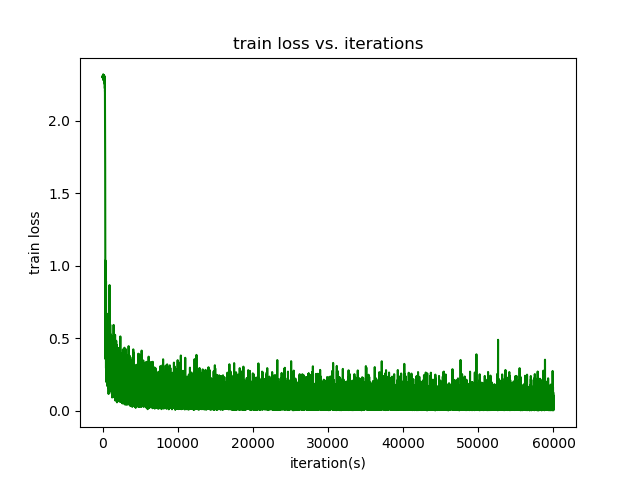
\includegraphics[width=\textwidth]{../results/trainloss1}
	\end{minipage}
	\begin{minipage}[t]{0.48\textwidth}
		\centering
		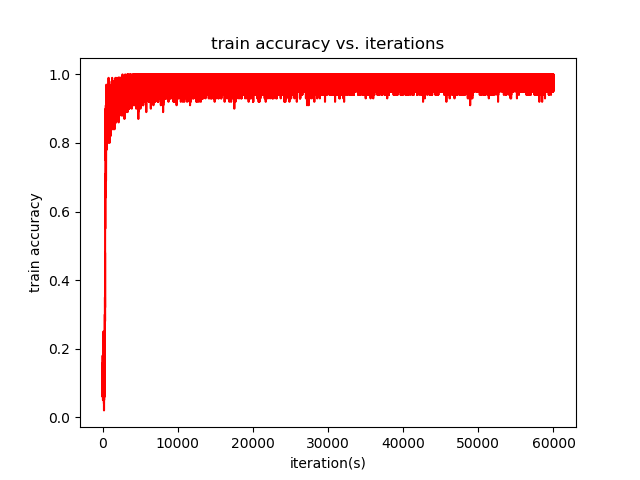
\includegraphics[width=\textwidth]{../results/trainacc1}
	\end{minipage}
	\caption{\label{trainres1}train loss curve and train accuracy curve in Experiments1}
\end{figure}

\begin{figure}[!h]
	\centering
	\begin{minipage}[t]{0.48\textwidth}
		\centering
		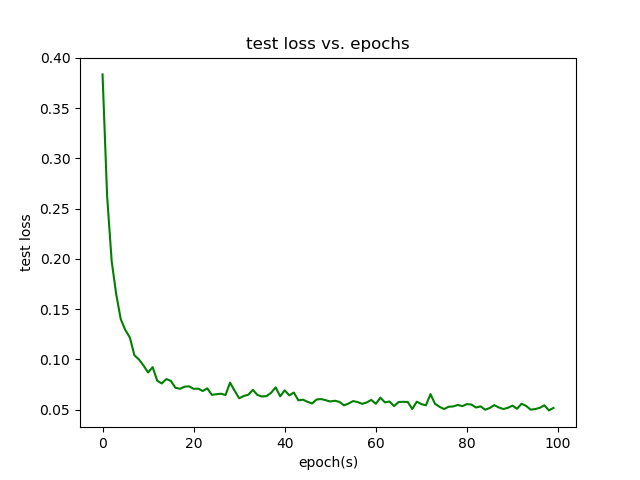
\includegraphics[width=\textwidth]{../results/testloss1}
	\end{minipage}
	\begin{minipage}[t]{0.48\textwidth}
		\centering
		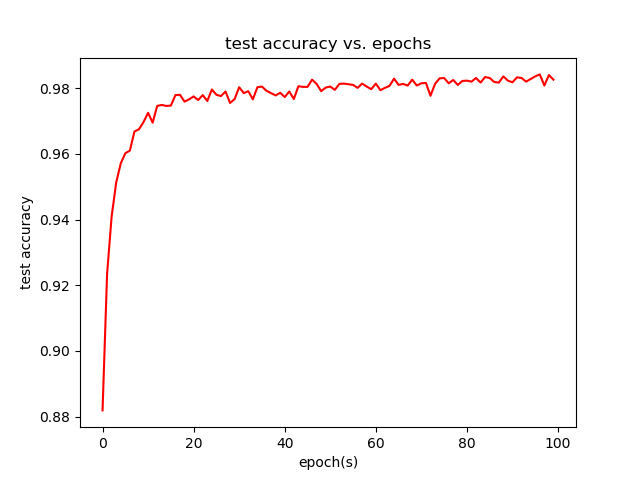
\includegraphics[width=\textwidth]{../results/testacc1}
	\end{minipage}
	\caption{\label{testres1}test loss curve and test accuracy curve in Experiments1}
\end{figure}
%\begin{table}[!ht]
%	\centering
%	\caption{\label{tab1}Network Structure with one hidden layer}
%	\begin{tabular}{|c|c|c|c|c|c|}
%		\hline
%		layer name & Input & Linear & Activation & Linear & Loss \\
%		\hline
%		\multirow{2}{*}{Size} & \multirow{2}{*}{$784 \times 1$} & \multirow{2}{*}{$784 \times 128$} & Relu & \multirow{2}{*}{$128\times 10$} &  EuclideanLoss \\
%		 & & & Sigmoid & &SoftmaxCrossEntropyLoss \\
%		\hline
%	\end{tabular}
%\end{table}



\section{Two hidden layers experiments}
The network structure in this section is designed as Table\ref{tab2} and training arguments is as follow:

\begin{lstlisting}[frame=single,language=python]  
config = {
    'learning_rate': 0.1,
    'weight_decay': 0.0001,
    'momentum': 0.9,
    'batch_size': 100,
    'max_epoch': 100,
    'disp_freq': 50,
}
\end{lstlisting}

\begin{figure}[htbp]
	\centering
	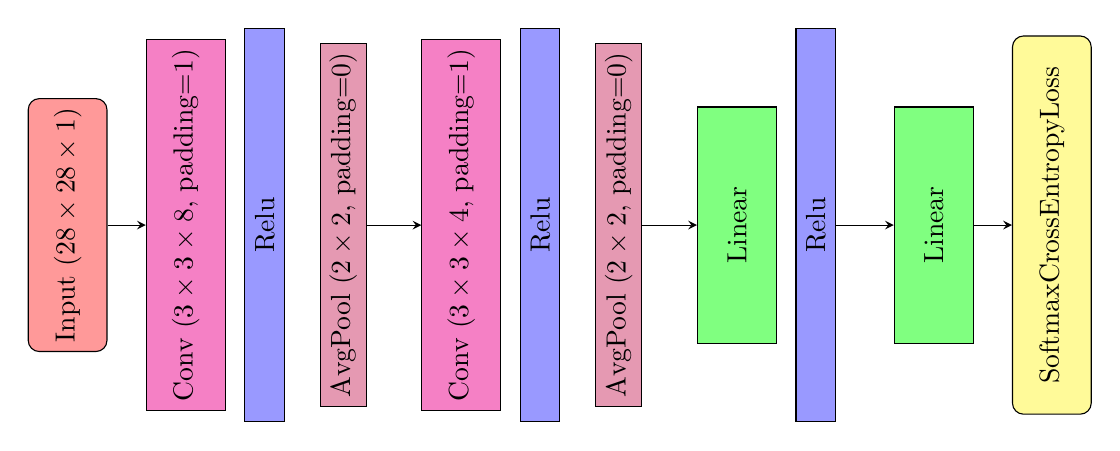
\begin{tikzpicture}
	\node (start) [startstop, rotate=90] {Input ($28\times28\times 1$)};
	\node (conv1) [conv, rotate=90, below of=start, yshift=-0.5cm] {Conv ($3\times3\times 8$, padding=1)};
	\node (acti1) [acti, rotate=90, below of=conv1] {Relu};
	\node (pool1) [pool, rotate=90, below of=acti1] {AvgPool ($2\times2$, padding=0)};
	\node (conv2) [conv, rotate=90, below of=pool1, yshift=-0.5cm] {Conv ($3\times3\times 4$, padding=1)};
	\node (acti2) [acti, rotate=90, below of=conv2] {Relu};
	\node (pool2) [pool, rotate=90, below of=acti2] {AvgPool ($2\times2$, padding=0)};
	\node (linear1) [process, rotate=90, below of=pool2, yshift=-0.5cm] {Linear};
	\node (acti3) [acti, rotate=90, below of=linear1] {Relu};
	\node (linear2) [process, rotate=90, below of=acti3, yshift=-0.5cm] {Linear};
	\node (loss) [loss, rotate=90, below of=linear2, yshift=-0.5cm, text width=13em] {SoftmaxCrossEntropyLoss};
	
	\draw [arrow](start) -- (conv1);
	%		\draw [arrow](conv1) -- (acti1);
	%		\draw [arrow](acti1) -- (pool1);
	\draw [arrow](pool1) -- (conv2);
	%		\draw [arrow](conv2) -- (acti2);
	%		\draw [arrow](acti2) -- (pool2);
	\draw [arrow](pool2) -- (linear1);
	\draw [arrow](acti3) -- (linear2);
	\draw [arrow](linear2) -- (loss);
	\end{tikzpicture}
	\caption{\label{fig2}Experiments2 Network Structure}
\end{figure}
%\begin{table}[!ht]
%	\centering
%	\caption{\label{tab2}Network Structure with two hidden layers}
%	\begin{tabular}{|c|c|c|c|}
%		\hline
%		layer name & Input & Linear & Activation  \\
%		\hline
%		\multirow{2}{*}{Size} & \multirow{2}{*}{$784 \times 1$} & \multirow{2}{*}{$784 \times 128$} & Relu \\
%		& & & Sigmoid  \\
%		\hline
%		Linear & Activation & Linear &Loss \\
%		\hline
%		\multirow{2}{*}{$128\times 64$} &  Relu & \multirow{2}{*}{$64\times 10$} &EuclideanLoss \\
%		& Sigmoid & &SoftmaxCrossEntropyLoss \\
%		\hline 
%	\end{tabular}
%\end{table}

\section{Results}
We summarize all test accuracys and test losses of every experiments as shown in Table \ref{tab3}(In this table, RE represents the experiments using Relu activation function and EuclideanLoss, SE represents the experiments using Sigmoid activation function and EuclideanLoss, RS represents the experiments using Relu activation function and SoftmaxCrossEntropyLoss, SS represents the experiments using Sigmoid activation function and SoftmaxCrossEntropyLoss). From the results, we can find the best chance is the experiments that use Relu activation function and EuclideanLoss with two hidden layers, the test accuracy is $0.983$.

\begin{table}[!ht]
	\centering
	\caption{\label{tab3}Results Summary}
	\begin{tabular}{|c|c|c|c|c|}
		\hline
		Cases & RE & SE & RS & SS \\
		\hline
		Test Acc with one hidden layer & 0.975 & 0.951 & 0.982 & 0.975 \\
		\hline
		Test Loss with one hidden layer & 0.039 & 0.062 & 0.062 & 0.083 \\
		\hline
		Test Acc with two hidden layers & {\color{red} 0.983} & 0.947 & 0.981 & 0.976 \\
		\hline
		Test Loss with two hidden layers & {\color{green} 0.021} & 0.053 & 0.065 & 0.075 \\
		\hline
	\end{tabular}
\end{table}

\end{document}